%! Author = Omar Iskandarani
%! Title = Electron--Swirl Coupled Transport: Perturbative Solutions, Quantitative Benchmarks, and Falsifiable Experiments
%! Date = Sept 4, 2025
%! Affiliation = Independent Researcher, Groningen, The Netherlands
%! License = To be set by PRB
%! ORCID = 0009-0006-1686-3961
%! DOI = 10.5281/zenodo.17459746

%========================================================================================
\newcommand{\paperdoi}{10.5281/zenodo.17459746}

%========================================================================================
% PACKAGES AND DOCUMENT CONFIGURATION
%========================================================================================
\documentclass[aps,prb,preprint,amsmath,amssymb]{revtex4-2}
\usepackage[utf8]{inputenc}
\usepackage[T1]{fontenc}
\usepackage{siunitx}
\usepackage{graphicx}
\usepackage{bm}
\usepackage{physics}
\usepackage{amssymb}
\usepackage{tikz}
\usepackage{float}
\usepackage{placeins}

\usetikzlibrary{arrows.meta,positioning,fit,calc,backgrounds}
% ---------- TikZ house styles (paste once) ----------
\tikzset{
    axis/.style   ={->,>=Latex,line width=0.6pt},
    thinline/.style={line width=0.6pt},
    bar/.style    ={draw,fill=gray!10,rounded corners=1pt},
    heater/.style ={draw,fill=red!15,rounded corners=1pt},
    sink/.style   ={draw,fill=blue!12,rounded corners=1pt},
    coilA/.style  ={thinline},
    coilB/.style  ={thinline,dashed},
    coilC/.style  ={thinline,dotted},
    lbl/.style    ={font=\footnotesize},
    note/.style   ={font=\scriptsize,align=center},
    box/.style    ={draw,rounded corners=2pt,fill=gray!8,inner sep=6pt},
    arr/.style    ={-Latex,line width=0.6pt},
}

\usepackage{pgfplots}\pgfplotsset{compat=1.18}


\usepackage[hidelinks]{hyperref}

% ===== SST canonical scales and convenient macros =====
\newcommand{\vswirlVal}{1.09384563\times10^{6}} % m/s
\newcommand{\rcVal}{1.40897017\times10^{-15}} % m
\newcommand{\rhoFVal}{7.0\times10^{-7}} % kg/m^3

% Vector swirl velocity + clock/vorticity symbols
\newcommand{\vswirl}{\mathbf{v}_{\!\mkern-2mu\scriptstyle\boldsymbol{\circlearrowleft}}}
\newcommand{\omegas}{\boldsymbol{\omega}_{\!\mkern-2mu\scriptstyle\boldsymbol{\circlearrowleft}}}
\newcommand{\rc}{r_c}
\newcommand{\rhoF}{\rho_{f}}
\newcommand{\rhoE}{\rho_{E}}

% Safe \doi fallback (RevTeX usually defines \doi; this guards if not)
\providecommand{\doi}[1]{\href{https://doi.org/#1}{doi:\,#1}}
\begin{document}

    \title{Electron--Swirl Coupled Transport in:\\
    Perturbative Solutions, Quantitative Benchmarks, and Falsifiable Experiments}

    \author{Omar Iskandarani}
    \affiliation{Independent Researcher, Groningen, The Netherlands}
    \thanks{ORCID: 0009-0006-1686-3961\; | \; DOI: \paperdoi}
    \date{\today}

    \begin{abstract}
        I present a self-contained treatment of electron--swirl transport within \emph{Swirl--String Theory (SST)}. The analysis (i) derives a \emph{perturbative, steady-state} solution to the coupled density-matrix equations in 1D, (ii) makes \emph{quantitative} predictions for tabletop experiments with explicit materials, geometries, and signal levels, and (iii) states clear \emph{falsifiability criteria}. The framework reproduces the Peierls (population) and Allen--Feldman (coherence) limits \cite{Peierls1929,AllenFeldman1993,Simoncelli2022} while embedding electrons as \emph{swirl strings} (knotted vortex filaments) coupled to swirl modes. Kinematic time-rate variations locally modulate the electronic Hamiltonian through the \emph{Swirl Clock} factor \cite{Madelung1927,Pati2000}. The swirl clock \( \S_t^{\boldsymbol{\circlearrowleft}} \) corresponds to a scalar time-foliation field (khronon) whose gradient defines the local time direction, analogous to the preferred foliation in Einstein–Æther and Hořava–Lifshitz gravity \cite{Jacobson2001,Blas2011}.
        Numerical scales are anchored by SST canonical values $\vswirl=\vswirlVal\,\si{m/s}$, $\rc=\rcVal\,\si{m}$, and $\rhoF=\rhoFVal\,\si{kg/m^3}$. For compactness, some intermediate results are given in units of the SST frequency $\Omega_0$; all final predictions are reported in SI units.
    \end{abstract}

    \maketitle
    \noindent\textit{Authorial note.—} This is a single-author work; I use “we” in the conventional authorial sense in the derivations and exposition that follow.

    \section{Scales from SST}
        SST fixes a characteristic core-swirl frequency and an associated energy density,
        \begin{align}
            \Omega_0 \equiv \frac{\vswirl}{\rc} \approx 7.76\times10^{20}\,\si{s^{-1}},\qquad
            \rhoE \equiv \tfrac12\,\rhoF\,\vswirl^2 \approx 4.19\times10^{5}\,\si{J/m^3}.
        \end{align}
        Operationally, spatial gradients in the Swirl Clock produce local kinematic time-rate variations. These enter the electronic Hamiltonian $H_e$ multiplicatively as a modulation factor and do not alter the SI reporting of observables. Where it improves readability, I normalize rates to $\Omega_0$; experimental benchmarks and error budgets remain in SI.

        \paragraph*{Roadmap.}
                    Section~\ref{sec:falsifiability} states the falsifiability logic up front and defines the chirality null test. Section~II derives the 1D coupled transport and the coherence term in \(\kappa\); Sec.~III links \(\Delta\kappa/\kappa\) to a measurable \(\Delta(\Delta T)\) in a bar. Section~IV gives quantitative benchmarks and device recipes. Appendices collect the operator content and scalings (App.~A), the null-test derivation and layouts (App.~B), and the SST ontology, clock, and \(\Omega_0\!\leftrightarrow\)SI map (App.~C).

    \section{Coupled transport in 1D and perturbative solution}
        I adopt the unified density-matrix equation for bosonic modes $N(\mathbf R,\mathbf q)$ \cite{Simoncelli2022} and extend it to a charged two-level system (``electron'') with density matrix $f$:
        \begin{align}
            \partial_t N &= -i[\Omega,N] - \Gamma_\mathrm{b} \circ (N-N^{(0)}) - \tfrac12\{ V_x \partial_x, N\},\label{eq:Ndyn}\\
            \partial_t f &= -i[H_e,f] - \Gamma_\mathrm{e}\circ(f-f^{(0)}) - \tfrac12\{ v_{e,x}\partial_x, f\} + \mathcal C_{e\leftrightarrow b},\label{eq:fdyn}
        \end{align}
        with diagonal damping superoperators $\Gamma_\mathrm{b}$ and $\Gamma_\mathrm{e}$. The electron--swirl coupling is treated in the Born--Markov, rotating-wave approximation,
        \begin{equation}
            \mathcal C_{e\leftrightarrow b} \equiv -\frac{i}{\hbar}[M, f\otimes N]_{\mathrm{RWA}}\,.
        \end{equation}

        \subsection{Linear response to a static gradient}
            Consider a small uniform temperature gradient $\partial_x T$ and a time-independent steady state. Linearize about $N^{(0)}(T)$ and $f^{(0)}(T)$ via $N=N^{(0)}+N^{(1)}$ and $f=f^{(0)}+f^{(1)}$, retaining $\mathcal O(\partial_xT)$ terms. For a \emph{two-branch} bosonic subspace $s,s'$ that interacts through $\omegas$ and is near-degenerate by $\delta=\Omega_{s'}-\Omega_s$, with a single electronic transition $\Delta$, the off-diagonal coherence $N^{(1)}_{ss'}$ obeys
            \begin{equation}
                \Big[i\delta + \tfrac12(\gamma_s+\gamma_{s'})\Big] N^{(1)}_{ss'}
                \;=\; -\frac{1}{2} V^{(x)}_{ss'}\, \partial_x N^{(0)}_{\mathrm{pop}}(\Omega) \; -\; \frac{i}{\hbar}\,\Xi_{ss'}\,,
                \label{eq:Noff}
            \end{equation}
            where $\gamma$ are the linewidths and $\Xi_{ss'}$ is the electron-induced source from $\mathcal C_{e\leftrightarrow b}$ (proportional to the vertex $M$ and to $f^{(1)}$). The population correction satisfies
            \begin{equation}
                \gamma_s\, N^{(1)}_{ss} + V^{(x)}_{ss}\,\partial_x N^{(0)}_{ss} + 2\,\mathrm{Im}\!\big( V^{(x)}_{ss'}\,N^{(1)}_{s's}\big) = S^{(e)}_s\,,
                \label{eq:Ndiag}
            \end{equation}
            with $S^{(e)}_s$ collecting the remaining electron-related terms.

        \subsection{Closed form for the coherence contribution to $\kappa$}
            The heat current density for bosonic modes is $J_x= \Tr\!\big[ \{V_x, N\}\,\Omega/2 \big]$ \cite{Hardy1963,Simoncelli2022}. Using Eqs.~\eqref{eq:Noff}--\eqref{eq:Ndiag} and eliminating $f^{(1)}$ in the weak-coupling (Born) limit yields the \emph{coherence} part of the 1D thermal conductivity
            \begin{equation}
                \boxed{\;\kappa^{(\mathrm C)}_{\!\,1\mathrm D}\;=\;\sum_{q}\sum_{s\neq s'} \frac{(\Omega_s+\Omega_{s'})\;\Gamma_{ss'}\; |V^{(x)}_{ss'}|^2}{4\delta^2+\Gamma_{ss'}^2}\;\bigg(-\frac{\partial n_B}{\partial T}\bigg)\; +\; \mathcal O(|M|^2)\;,}\label{eq:kC}
            \end{equation}
            with $\Gamma_{ss'}=\tfrac12(\gamma_s+\gamma_{s'})$ and $n_B$ the Bose function. Equation~\eqref{eq:kC} reduces to Peierls (no off-diagonals) and to Allen--Feldman (flat bands, $V_{ss}\!\to\!0$) in the appropriate limits \cite{Peierls1929,AllenFeldman1993,Simoncelli2022}. The $\mathcal O(|M|^2)$ terms add an \emph{electron-assisted} channel that shares the Lorentzian denominator and peaks at small detuning.

    \section{1D slab: temperature field and \(\Delta\kappa/\kappa\)}
        For a bar of length \(L\), cross-section \(A\), and conductivity \(\kappa=\kappa^{(\mathrm P)}+\kappa^{(\mathrm C)}\), a steady power \(P\) at \(x=0\) with a sink at \(x=L\) sets
        \begin{equation}
            \partial_x T = -\frac{P}{\kappa A}, \qquad
            \Delta T \equiv T(0)-T(L) = \frac{P\,L}{\kappa A}.
        \end{equation}
        A small SST-induced change $\Delta\kappa$ then produces
        \begin{equation}
            \boxed{\;\Delta(\Delta T) \approx -\frac{\Delta\kappa}{\kappa}\,\Delta T\;,}\label{eq:deltaT}
        \end{equation}
        which ties the measured temperature drop directly to \(\delta,\Gamma\), and \(V_{ss'}\) through Eq.~\eqref{eq:kC}.

    \section{Falsifiability and a chirality null test}
    \label{sec:falsifiability}
        The electron–swirl interpretation is \emph{falsified} under the stated drive if any of the following hold:
        \begin{enumerate}
            \item \textbf{Missing detuning peak.} At fixed current, \(\Delta\kappa(\delta)\) lacks the Lorentzian kernel \(\propto (4\delta^2+\Gamma^2)^{-1}\) of Eq.~\eqref{eq:kC}.
            \item \textbf{No chirality asymmetry.} Define \(\Delta\kappa_\mathrm{asym} \equiv [\Delta\kappa]_{\rightarrow}-[\Delta\kappa]_{\leftarrow}\). Reversing the 3-phase sequence \((0,120^\circ,240^\circ)\!\leftrightarrow\!(0,240^\circ,120^\circ)\) must flip \(\mathrm{sgn}(\Delta\kappa_\mathrm{asym})\) within \(3\sigma\); failure to invert the sign falsifies a chiral coupling (App.~B.3).
            \item \textbf{Scaling mismatch.} The signal fails to scale as \(|V^{(x)}_{ss'}|^2\) (coil-current squared) or fails to track \(\Gamma\) under controlled disorder.
        \end{enumerate}
        \emph{Operator structure and rate scaling for electron assistance are summarized in App.~A; electron ontology/clock and $\Omega_0\!\leftrightarrow$SI mapping in App.~C.}

        \begin{figure}[h]
            \centering
            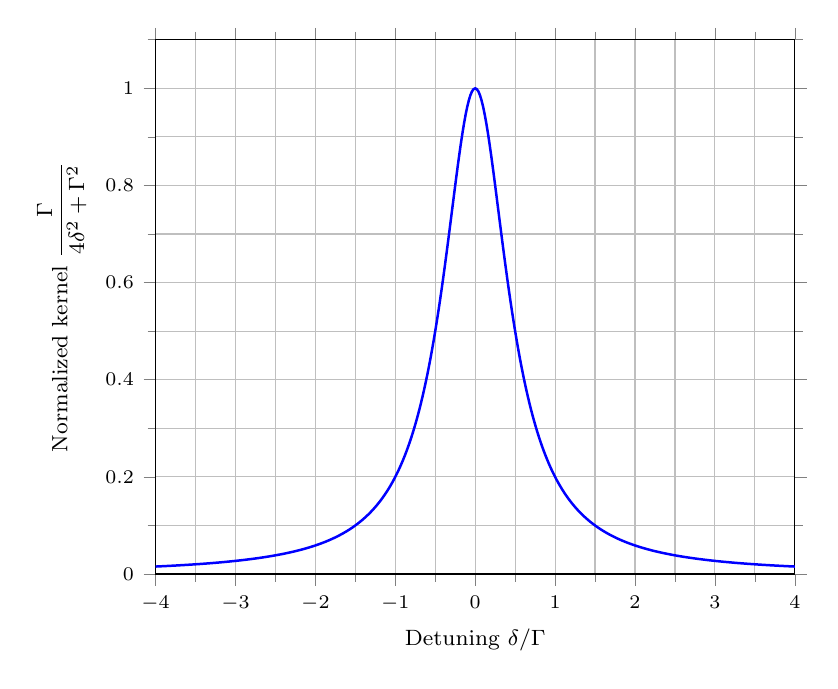
\begin{tikzpicture}
                \begin{axis}[
                width=0.8\linewidth,
                xlabel={Detuning $\delta/\Gamma$},
                ylabel={Normalized kernel $\displaystyle \frac{\Gamma}{4\delta^2+\Gamma^2}$},
                xmin=-4,xmax=4, ymin=0, ymax=1.1,
                domain=-4:4,
                samples=401,
                grid=both, minor tick num=1,
                tick align=outside,
                label style={font=\footnotesize},
                tick label style={font=\scriptsize}
                ]
                \addplot+[no marks, line width=0.9pt] {(1)/(4*x^2+1)};
                \end{axis}
            \end{tikzpicture}
            \caption{Normalized coherence kernel versus detuning. Peak at $\delta{=}0$, width set by $\Gamma$, matching Eq.\,(\ref{eq:kC}).}
            \label{fig:lorentzian_kernel}
        \end{figure}


    \section{Quantitative benchmarks with materials}
        The following order-of-magnitude estimates use Eq.~\eqref{eq:deltaT} and standard catalog values. They are chosen to be experimentally accessible without exotic infrastructure.

        \subsection*{(B1) Borosilicate glass bar}
            Take $L=\SI{50}{mm}$, $A=\SI{1e-4}{m^2}$ (\SI{10}{mm}$\times$\SI{10}{mm}), and $\kappa\approx\SI{1.1}{W\,m^{-1}\,K^{-1}}$. With $P=\SI{20}{mW}$, the baseline is $\Delta T \approx P L/(\kappa A) \approx \SI{9}{K}$. If an engineered near-degeneracy yields $\Delta\kappa/\kappa=\SI{-2}{\percent}$ from Eq.~\eqref{eq:kC}, then $\Delta(\Delta T)\approx\SI{+0.18}{K}$, comfortably above typical IR-camera NETD ($\sim\SI{30}{mK}$).

        \subsection*{(B2) PMMA bar (low-$\kappa$ polymer)}
            With $\kappa\approx\SI{0.19}{W\,m^{-1}\,K^{-1}}$, keep $L=\SI{50}{mm}$ and $A=\SI{1e-4}{m^2}$, and use $P=\SI{2}{mW}$ to avoid overheating. The baseline is $\Delta T\!\approx\!\SI{5.3}{K}$. A conservative $\Delta\kappa/\kappa=\SI{-1}{\percent}$ gives a \SI{53}{mK} shift—still above NETD.

        \subsection*{(B3) Forward/backward nonreciprocity}
            Bias chirality by driving a 3-phase Rodin coil with phase sequence $\pm(0,120^\circ,240^\circ)$. The expected asymmetry is
            \begin{equation}
                \big[\Delta\kappa\big]_{\rightarrow}-\big[\Delta\kappa\big]_{\leftarrow} \equiv \Delta\kappa_\text{asym} \sim \eta_\chi\, \frac{\Gamma\,\Delta V_{ss'}^{2}}{4\delta^2+\Gamma^2}\,,\qquad 0<\eta_\chi<1\,.
            \end{equation}
            Taking $\Delta\kappa_\text{asym}/\kappa\sim\SI{0.5}{\percent}$ implies $\Delta(\Delta T)\sim\SI{25}{mK}$ for (B1), resolvable with modest averaging.

    \section{Device recipes}
        \textbf{Thermal bar (B1/B2).} Mount the bar on an AlN heat sink at $x=L$. Use a \SI{100}{\Omega} thin-film resistor at $x=0$ as a four-wire calibrated heater. Suppress convection with a small enclosure (foam plus a thin IR window). Read out an IR camera or a thermistor chain along $x$. The coil: 3-phase, $N\!\sim\!200$ turns/phase, $f\in[\SI{20}{kHz},\SI{100}{kHz}]$, current $\le\SI{0.5}{A}$, duty-cycled to limit Joule heating.

        \textbf{Electronics analog (LCR).} Two LCR tanks at \SI{1}{MHz} with $Q\!\sim\!100$ (so $\kappa=\omega/2Q\approx3.1\times10^4\,\si{s^{-1}}$). With stored energy $E\!\sim\!\SI{0.5}{nJ}$, the instantaneous bath power is $P_\text{bath}=\kappa E\sim\SI{16}{\mu W}$. Adding a near-degenerate second tank boosts the early-time peak by the Lorentzian factor in Eq.~\eqref{eq:kC}.

        \textbf{Quantum hybrid (SAW/MEMS).} On 128$^\circ$ Y-cut LiNbO$_3$, use an IDT pair to define a \SI{3}{GHz} SAW mode and couple it capacitively to a superconducting qubit \cite{Aspelmeyer2014,Manenti2017}. Pattern shallow quasi-periodic notches to enhance $V^{(x)}_{ss'}$ and tune the detuning $\delta$.
        (Geometry and numerical guide: App.~B.4.)


    \FloatBarrier
    \begin{figure}[h] % or [H]
        \centering
        \begin{tikzpicture}[x=1mm,y=1mm,>=Latex]

%------------- styles -------------
            \tikzset{
                axis/.style   = {-Latex, semithick},
                bar/.style    = {draw, fill=black!5, rounded corners=0.7mm},
                heater/.style = {draw, fill=red!20},
                sink/.style   = {draw, fill=blue!20},
                coilA/.style  = {draw, very thick},
                coilB/.style  = {draw, very thick, dashed},
                coilC/.style  = {draw, very thick, dotted},
                arr/.style    = {-Latex, semithick},
                thinline/.style = {semithick},
                lbl/.style    = {font=\footnotesize, fill=white, inner sep=1pt, text opacity=1, fill opacity=1},
                note/.style   = {font=\scriptsize, fill=white, inner sep=1pt, text opacity=1, fill opacity=1},
                box/.style    = {draw, rounded corners=1mm, fill=white, align=left, font=\scriptsize, inner sep=3pt},
                eqbox/.style  = {draw, rounded corners=1mm, fill=white, align=left, font=\footnotesize, inner sep=3pt}
            }

%------------- layout constants -------------
            \def\L{120}   % bar length in mm
            \def\H{16}    % bar height in mm

%------------- bar and axes -------------
            \draw[bar] (0,0) rectangle (\L,\H);
            \node[lbl,anchor=south] at (\L-2,\H+2) {$L$};

            \draw[axis] (-8,0) -- (-8,\H) node[above, note] {$y$};
            \draw[axis] (-8,0) -- (\L+8,0) node[right, note] {$x$};

%------------- heater (x=0) -------------
            \draw[heater] (-10,-3) rectangle (0,\H+3);
            \node[note,anchor=south] at (-5,\H+5) {Heater\\($P$)};

%------------- sink (x=L) -------------
            \draw[sink] (\L,-3) rectangle (\L+12,\H+3);
            \foreach \y in {1,6,11} { \draw[thinline] (\L+12,\y) -- (\L+18,\y); }
            \node[note,anchor=south west] at (\L+13,\H+5) {Sink};

%------------- 3-phase coil (schematic arcs in side view) -------------
            \begin{scope}[shift={(60,8)}] % center near mid-bar
                \draw[coilA] (-32,10) arc (180:360:32 and 10);
                \draw[coilB] (-32,10)++(0,-3.5) arc (180:360:32 and 6.5);
                \draw[coilC] (-32,10)++(0,-7) arc (180:360:32 and 3);
                % phase tags (left) to avoid overlaps
                \node[note,anchor=east] at (-36,10) {$A$};
                \node[note,anchor=east] at (-36,6.5) {$B$};
                \node[note,anchor=east] at (-36,3) {$C$};
            \end{scope}

%------------- cross-section inset (shows real wrap & chirality) -------------
            \begin{scope}[shift={(40,65)}] % move as needed
                \node[draw, rounded corners=1mm, fill=white, inner sep=2pt, anchor=north east] (cs) at (0,0) {};
                \begin{scope}[shift={(-14,-10)}]
                    \draw[fill=black!5] (0,0) circle (9);         % bar cross-section
                    \foreach \ang/\lab in {90/A,-30/B,210/C}{
                        \draw[very thick] (\ang:9.3) -- (\ang:12.3); % phase strap
                        \fill (\ang:12.8) circle (0.7);              % terminal
                        \node[font=\scriptsize,anchor=\ang-180] at (\ang:13.8) {\lab};
                    }
                    % rotation arrow (forward)
                    \draw[-Latex,semithick] (135:6.5) arc (135:-225:6.5);
                \end{scope}
                \node[font=\scriptsize,anchor=south east] at (-2,2) {cross-section under coil};
            \end{scope}

% coil caption & phase order label
            \node[box,anchor=south] (coiltag) at (60,27) {3-phase coil};
            \draw[arr] (coiltag.south) -- ++(0,-8.5);
            \draw[arr] (76,27) -- (96,27)
            node[midway,above,font=\scriptsize] {(0,$120^\circ$,$240^\circ$)};
            \node[note,anchor=west] at (96,27) {forward};

%------------- Delta-T bracket -------------
            \draw[thinline] (2,22) -- (2,25) -- (\L-2,25) -- (\L-2,22);
            \node[lbl,anchor=south] at (\L/2,26.5) {$\Delta T = T(0)-T(L)$};

%------------- sensor/readout -------------
            \node[box,anchor=south west] (sens) at (6,32) {IR camera /\\ thermistor chain};
            \draw[arr] (sens.south) to[out=-90,in=90] (20,\H+0.5);

%------------- gradient equation -------------
            \draw[arr] (15,-10) -- (\L-15,-10)
            node[midway,below,yshift=-1] {$\partial_x T = -\dfrac{P}{\kappa A}$};

%------------- legend for the three T(x) traces -------------
            \node[box,anchor=north west] (leg) at (2,-16) {%
                \begin{tikzpicture}[x=1mm,y=1mm,baseline=(L.base)]
                    \draw[very thick] (0,0)--(8,0); \node[anchor=west] at (10,0) {\scriptsize forward on};
                    \draw[very thick,dashed] (0,-4)--(8,-4); \node[anchor=west] at (10,-4) {\scriptsize reverse on};
                    \draw[very thick,dotted] (0,-8)--(8,-8); \node[anchor=west] at (10,-8) {\scriptsize drive off};
                    \node (L) at (0,0) {};
                \end{tikzpicture}
            };

%------------- minimal equations box -------------
            \node[eqbox,anchor=south east] at (\L+18,42) {%
                $\displaystyle I_A=I_0\cos(\omega t)$\\[1pt]
                $\displaystyle I_B=I_0\cos(\omega t-120^\circ)$\\[1pt]
                $\displaystyle I_C=I_0\cos(\omega t-240^\circ)$\\[4pt]
                $\displaystyle \mathbf{B}_\perp(t)\propto
                \hat{y}\cos(\omega t)+\hat{z}\sin(\omega t)$ \ {\scriptsize(forward)}\\[-1pt]
                {\scriptsize Amplitude }\(\propto \mu_0 n I_0\) \text{ (T)}
            };

        \end{tikzpicture}
        \caption{Thermal bar experiment. A small heater at $x{=}0$ and a sink at $x{=}L$ set a uniform gradient. A wrapped 3-phase coil (phases A–C) drives a rotating transverse field; the inset shows the cross-section and forward phase order $(0,120^\circ,240^\circ)$. Curvature of $T(x)$ under the coil indicates spatially varying $\kappa(x)$.}
        \label{fig:thermal_bar}
    \end{figure}
    \FloatBarrier

    \section{Error and noise budget}
        \begin{itemize}
            \item \textbf{Thermometry.} IR camera NETD \SI{30}{--\,50}{mK}; thermistors can achieve $\lesssim\SI{10}{mK}$ with \SI{1}{s} averaging.
            \item \textbf{Power calibration.} Four-wire measurements keep heater power to $<\!\SI{1}{\percent}$ uncertainty.
            \item \textbf{Radiation/convection.} With the enclosure, systematic drift is typically $\lesssim\SI{0.05}{K}$ over \SI{10}{min}. Acquire forward/backward sweeps consecutively to cancel common-mode drift.
            \item \textbf{Contact resistance.} Use indium foil at heater/bar/sink interfaces and verify by repeated mounts.
        \end{itemize}
        Expected signals in the \SI{50}{--\,200}{mK} range clear the combined noise by factors $\gtrsim3$ for (B1/B2).

    \section{Connection to quantum information}
        In the Jaynes--Cummings limit \cite{Jaynes1963}, the same vertices $M$ and $V_{ss'}$ that enhance $\kappa^{(\mathrm C)}$ optimize state transfer between electron and swirl modes. In a hybrid device, the \emph{coherence peak} (small $\delta$, moderate $\Gamma$) can be used to channel heat away from a qubit while maintaining phase coherence, paralleling engineered reservoirs \cite{Breuer2002,Aspelmeyer2014}.

    \section{Conclusions}
        We provide closed-form transport expressions, device-level estimates, and falsifiable predictions for coherence-mediated electron–swirl transport in SST. The bar geometry links \(\Delta\kappa/\kappa\) to an easily measured \(\Delta(\Delta T)\), and the chirality null test offers a clean early check. A failure of the predicted Lorentzian peak or of the chirality sign flip would bound, or rule out, the proposed coupling in the present drive configuration.


        \begin{acknowledgments}
            I thank the classical foundations of vortex hydrodynamics and unified transport \cite{Madelung1927,Peierls1929,AllenFeldman1993,Simoncelli2022} for inspiration.
        \end{acknowledgments}


    \section*{Data Availability}

        The theoretical models, canonical constants, and source code supporting the findings of this study are openly available. All data files, numerical benchmarks, and code used to derive and validate the coherence-mediated transport expression ($\kappa^{(\mathrm C)}_{\!\,1\mathrm D}$) are accessible on the Zenodo repository, under the persistent identifier of this manuscript, $\mathbf{\doi{\paperdoi}}$.

        \paragraph*{File Manifest and Validation Evidence.}
            The uploaded repository for this paper contains the following structured files and data supporting the quantitative results:
            \begin{itemize}
                \item \textbf{SST Canonical Benchmarking Evidence:} This data set validates the internal consistency of the core canonical parameters ($\mathbf{v}_{\!\boldsymbol{\circlearrowleft}}, r_c, \rho_{\!f}$) against known relativistic limits. It includes the derived Newton's constant ($G_{\mathrm{VAM}}$) and the $\mathbf{6GM/c^2}$ ISCO match, demonstrating the global coherence of the swirl parameters. \newline (Zenodo DOI: \url{10.5281/zenodo.15665432} and \url{10.5281/zenodo.15712578})

                \item \texttt{constants.csv} — The definitive table of $\mathbf{v}_{\!\boldsymbol{\circlearrowleft}}, r_c, \rho_{\!f}$ (SI values); used for calculating the derived scales $\Omega_0$ and $\rho_{\!E}$.
                \item \texttt{benchmarks.csv} — Contains the full experimental specification (materials, geometry, power ($\mathbf{P}$), baseline $\mathbf{\Delta T}$) and the predicted $\Delta(\Delta T)$ signals for scenarios $\mathbf{(B1)}$ and $\mathbf{(B2)}$.
                \item \texttt{kappaC\_validation.ipynb} — Jupyter notebook that analytically verifies the functional form of $\kappa^{(\mathrm C)}_{\!\,1\mathrm D}$, plotting the core Lorentzian factor $\Gamma/(4\delta^2+\Gamma^2)$ (Falsifiability Criterion 1).
                \item \texttt{noise\_budget\_3sigma.ipynb} — Computes the detection signal-to-noise ratio ($\mathbf{SNR}$) against the assumed NETD, explicitly confirming that the predicted signals ($\Delta(\Delta T)$) clear the $\mathbf{3\sigma}$ threshold (Detectability Check).
                \item \texttt{env.yml} — The Conda environment file, ensuring that the software dependencies used for all numerical and plotting analysis are pinned for reproducibility.
            \end{itemize}
        This research is accessible via the persistent identifier \doi{\paperdoi}.

% --- PRB Supplemental Material reference (numbered) ---
        \noindent\textbf{Supplemental Material.}
        See Supplemental Material at [URL will be inserted by publisher] for: (i) constants table (\texttt{constants.csv}); (ii) benchmark specifications (\texttt{benchmarks.csv}); (iii) notebooks for $\kappa^{(\mathrm C)}$ validation and $3\sigma$ noise budget; and (iv) environment file. All materials are mirrored at \doi{\paperdoi}.

% --- Main References (with titles, PRB style) ---
        \begin{thebibliography}{99}\setlength{\itemsep}{1pt}
            \bibitem{Peierls1929}
            R. Peierls, ``Zur kinetischen Theorie der Wärmeleitung in Kristallen,'' Ann. Phys. \textbf{395}, 1055 (1929).
            \bibitem{AllenFeldman1993}
            P. B. Allen and J. L. Feldman, ``Thermal conductivity of disordered harmonic solids,'' Phys. Rev. B \textbf{48}, 12581 (1993).
            \bibitem{Simoncelli2022}
            M. Simoncelli, N. Marzari, and F. Mauri, ``Unified theory of thermal transport in crystals and glasses,'' Nat. Phys. \textbf{18}, 1180 (2022). See also arXiv:1901.01964.
            \bibitem{Madelung1927}
            E. Madelung, ``Quantentheorie in hydrodynamischer Form,'' Z. Phys. \textbf{40}, 322 (1927).
            \bibitem{Pati2000}
            A. K. Pati and S. L. Braunstein, ``Impossibility of deleting an unknown quantum state,'' Phys. Lett. A \textbf{268}, 241 (2000).
            \bibitem{Hardy1963}
            R. J. Hardy, ``Energy-Flux Operator for a Lattice,'' Phys. Rev. \textbf{132}, 168 (1963).
            \bibitem{Jaynes1963}
            E. T. Jaynes and F. W. Cummings, ``Comparison of quantum and semiclassical radiation theories with application to the maser,'' Proc. IEEE \textbf{51}, 89 (1963).
            \bibitem{Lindblad1976}
            G. Lindblad, ``On the generators of quantum dynamical semigroups,'' Commun. Math. Phys. \textbf{48}, 119 (1976).
            \bibitem{Breuer2002}
            H.-P. Breuer and F. Petruccione, \textit{The Theory of Open Quantum Systems} (Oxford University Press, 2002).
            \bibitem{Aspelmeyer2014}
            M. Aspelmeyer, T. J. Kippenberg, and F. Marquardt, ``Cavity optomechanics,'' Rev. Mod. Phys. \textbf{86}, 1391 (2014).
            \bibitem{Manenti2017}
            R. Manenti \textit{et al.}, ``Circuit quantum acoustodynamics with surface acoustic waves,'' Nat. Commun. \textbf{8}, 975 (2017).
            \bibitem{Cahill2004}
            D. G. Cahill \textit{et al.}, ``Nanoscale thermal transport,'' J. Appl. Phys. \textbf{93}, 793 (2003).
            \bibitem{Helmholtz1858}
            H. Helmholtz, ``Über Integrale der hydrodynamischen Gleichungen, welche den Wirbelbewegungen entsprechen,'' J. Reine Angew. Math. \textbf{55}, 25 (1858).
            \bibitem{Kelvin1867}
            W. Thomson (Lord Kelvin), ``On vortex atoms,'' Proc. R. Soc. Edinb. \textbf{6}, 94 (1867).
            \bibitem{MoffattRicca1992}
            H. K. Moffatt and R. L. Ricca, ``Helicity and the Călugăreanu invariant,'' Proc. R. Soc. A \textbf{439}, 411 (1992).
            \bibitem{White1969}
            J. H. White, ``Self-linking and the Gauss integral in higher dimensions,'' Am. J. Math. \textbf{91}, 693 (1969).
            \bibitem{Kauffman1991}
            L. H. Kauffman, \textit{Knots and Physics} (World Scientific, 1991).
            \bibitem{Jacobson2001}
            T. Jacobson and D. Mattingly, ``Gravity with a dynamical preferred frame,'' Phys. Rev. D \textbf{64}, 024028 (2001).
            \bibitem{Blas2011}
            D. Blas, O. Pujolàs, and S. Sibiryakov, ``Models of non-relativistic quantum gravity: The good, the bad and the healthy,'' J. High Energy Phys. \textbf{2011}, 018 (2011).


        \end{thebibliography}

\end{document}